% Options for packages loaded elsewhere
\PassOptionsToPackage{unicode}{hyperref}
\PassOptionsToPackage{hyphens}{url}
%
\documentclass[
]{article}
\usepackage{amsmath,amssymb}
\usepackage{lmodern}
\usepackage{iftex}
\ifPDFTeX
  \usepackage[T1]{fontenc}
  \usepackage[utf8]{inputenc}
  \usepackage{textcomp} % provide euro and other symbols
\else % if luatex or xetex
  \usepackage{unicode-math}
  \defaultfontfeatures{Scale=MatchLowercase}
  \defaultfontfeatures[\rmfamily]{Ligatures=TeX,Scale=1}
\fi
% Use upquote if available, for straight quotes in verbatim environments
\IfFileExists{upquote.sty}{\usepackage{upquote}}{}
\IfFileExists{microtype.sty}{% use microtype if available
  \usepackage[]{microtype}
  \UseMicrotypeSet[protrusion]{basicmath} % disable protrusion for tt fonts
}{}
\makeatletter
\@ifundefined{KOMAClassName}{% if non-KOMA class
  \IfFileExists{parskip.sty}{%
    \usepackage{parskip}
  }{% else
    \setlength{\parindent}{0pt}
    \setlength{\parskip}{6pt plus 2pt minus 1pt}}
}{% if KOMA class
  \KOMAoptions{parskip=half}}
\makeatother
\usepackage{xcolor}
\usepackage[margin=1in]{geometry}
\usepackage{color}
\usepackage{fancyvrb}
\newcommand{\VerbBar}{|}
\newcommand{\VERB}{\Verb[commandchars=\\\{\}]}
\DefineVerbatimEnvironment{Highlighting}{Verbatim}{commandchars=\\\{\}}
% Add ',fontsize=\small' for more characters per line
\usepackage{framed}
\definecolor{shadecolor}{RGB}{248,248,248}
\newenvironment{Shaded}{\begin{snugshade}}{\end{snugshade}}
\newcommand{\AlertTok}[1]{\textcolor[rgb]{0.94,0.16,0.16}{#1}}
\newcommand{\AnnotationTok}[1]{\textcolor[rgb]{0.56,0.35,0.01}{\textbf{\textit{#1}}}}
\newcommand{\AttributeTok}[1]{\textcolor[rgb]{0.77,0.63,0.00}{#1}}
\newcommand{\BaseNTok}[1]{\textcolor[rgb]{0.00,0.00,0.81}{#1}}
\newcommand{\BuiltInTok}[1]{#1}
\newcommand{\CharTok}[1]{\textcolor[rgb]{0.31,0.60,0.02}{#1}}
\newcommand{\CommentTok}[1]{\textcolor[rgb]{0.56,0.35,0.01}{\textit{#1}}}
\newcommand{\CommentVarTok}[1]{\textcolor[rgb]{0.56,0.35,0.01}{\textbf{\textit{#1}}}}
\newcommand{\ConstantTok}[1]{\textcolor[rgb]{0.00,0.00,0.00}{#1}}
\newcommand{\ControlFlowTok}[1]{\textcolor[rgb]{0.13,0.29,0.53}{\textbf{#1}}}
\newcommand{\DataTypeTok}[1]{\textcolor[rgb]{0.13,0.29,0.53}{#1}}
\newcommand{\DecValTok}[1]{\textcolor[rgb]{0.00,0.00,0.81}{#1}}
\newcommand{\DocumentationTok}[1]{\textcolor[rgb]{0.56,0.35,0.01}{\textbf{\textit{#1}}}}
\newcommand{\ErrorTok}[1]{\textcolor[rgb]{0.64,0.00,0.00}{\textbf{#1}}}
\newcommand{\ExtensionTok}[1]{#1}
\newcommand{\FloatTok}[1]{\textcolor[rgb]{0.00,0.00,0.81}{#1}}
\newcommand{\FunctionTok}[1]{\textcolor[rgb]{0.00,0.00,0.00}{#1}}
\newcommand{\ImportTok}[1]{#1}
\newcommand{\InformationTok}[1]{\textcolor[rgb]{0.56,0.35,0.01}{\textbf{\textit{#1}}}}
\newcommand{\KeywordTok}[1]{\textcolor[rgb]{0.13,0.29,0.53}{\textbf{#1}}}
\newcommand{\NormalTok}[1]{#1}
\newcommand{\OperatorTok}[1]{\textcolor[rgb]{0.81,0.36,0.00}{\textbf{#1}}}
\newcommand{\OtherTok}[1]{\textcolor[rgb]{0.56,0.35,0.01}{#1}}
\newcommand{\PreprocessorTok}[1]{\textcolor[rgb]{0.56,0.35,0.01}{\textit{#1}}}
\newcommand{\RegionMarkerTok}[1]{#1}
\newcommand{\SpecialCharTok}[1]{\textcolor[rgb]{0.00,0.00,0.00}{#1}}
\newcommand{\SpecialStringTok}[1]{\textcolor[rgb]{0.31,0.60,0.02}{#1}}
\newcommand{\StringTok}[1]{\textcolor[rgb]{0.31,0.60,0.02}{#1}}
\newcommand{\VariableTok}[1]{\textcolor[rgb]{0.00,0.00,0.00}{#1}}
\newcommand{\VerbatimStringTok}[1]{\textcolor[rgb]{0.31,0.60,0.02}{#1}}
\newcommand{\WarningTok}[1]{\textcolor[rgb]{0.56,0.35,0.01}{\textbf{\textit{#1}}}}
\usepackage{graphicx}
\makeatletter
\def\maxwidth{\ifdim\Gin@nat@width>\linewidth\linewidth\else\Gin@nat@width\fi}
\def\maxheight{\ifdim\Gin@nat@height>\textheight\textheight\else\Gin@nat@height\fi}
\makeatother
% Scale images if necessary, so that they will not overflow the page
% margins by default, and it is still possible to overwrite the defaults
% using explicit options in \includegraphics[width, height, ...]{}
\setkeys{Gin}{width=\maxwidth,height=\maxheight,keepaspectratio}
% Set default figure placement to htbp
\makeatletter
\def\fps@figure{htbp}
\makeatother
\setlength{\emergencystretch}{3em} % prevent overfull lines
\providecommand{\tightlist}{%
  \setlength{\itemsep}{0pt}\setlength{\parskip}{0pt}}
\setcounter{secnumdepth}{-\maxdimen} % remove section numbering
\ifLuaTeX
  \usepackage{selnolig}  % disable illegal ligatures
\fi
\IfFileExists{bookmark.sty}{\usepackage{bookmark}}{\usepackage{hyperref}}
\IfFileExists{xurl.sty}{\usepackage{xurl}}{} % add URL line breaks if available
\urlstyle{same} % disable monospaced font for URLs
\hypersetup{
  pdftitle={Causes of deaths by age in Switzerland},
  pdfauthor={Rachel Ferati},
  hidelinks,
  pdfcreator={LaTeX via pandoc}}

\title{Causes of deaths by age in Switzerland}
\author{Rachel Ferati}
\date{2022-12-14}

\begin{document}
\maketitle

{
\setcounter{tocdepth}{2}
\tableofcontents
}
This report uses the R programming language and the following R
libraries

\begin{Shaded}
\begin{Highlighting}[]
\FunctionTok{library}\NormalTok{(tidyverse)}
\FunctionTok{library}\NormalTok{(knitr)}
\FunctionTok{library}\NormalTok{(ggplot2)}
\FunctionTok{library}\NormalTok{(dplyr)}
\FunctionTok{library}\NormalTok{(treemap)}
\FunctionTok{library}\NormalTok{(hrbrthemes)}
\end{Highlighting}
\end{Shaded}

\hypertarget{introduction}{%
\section{Introduction}\label{introduction}}

\emph{How Am I going to die} ? We all one day ask ourselves this
question. And, of course, this question is often followed by \emph{When
Am I going to die ?}. The way we are going to die. Although these
questions cannot be answered, it is important to identify the number of
deaths and their causes to have a better understanding of the situation
in a country.

\begin{quote}
\begin{quote}
\begin{quote}
An important input to national and international health decision-making
and planning processes is a consistent and comparative analysis of the
causes of death across different population groups (Mathers, C.B.,
Boerma T., Ma Fat D. (2009))
\end{quote}
\end{quote}
\end{quote}

Indeed, the causes of death differ from one country to another, and also
from one person to another. It depends on many factors, i.e., the
social-economic environment, the age, the family, etc. It is important
for a family to know which disease occurs whithin the family, and it is
important for the country to know which are the causes of deaths of the
population. To know that, there are a lot of database that exist for
many countries. The one from which we extracted the data needed for our
essay comes from the World Health Organization
\href{@https://www.who.int/data/gho/data/themes/mortality-and-global-health-estimates/ghe-leading-causes-of-death}{WHO}

\begin{quote}
\begin{quote}
\begin{quote}
Over the last decade, the WHO has intensified efforts to support the
collection of vital registration information and other mortality data in
developing countries (Mathers, C.B., Boerma T., Ma Fat D. (2009))
\end{quote}
\end{quote}
\end{quote}

\hypertarget{research-question}{%
\subsection{Research question}\label{research-question}}

In this essay, we will be interested in the differences between the
three leading causes of death across ages, and more precisely between
children and adults. We will less focused on the number of death in
itslef, since it is not surprising that more people died when they get
older, but rather on the type of causes, whether it is communicable,
meaning that it is transmitted to one another (genetic ilnesses),
non-communicable and injuries, meaning the causes that comes from the
external world (car accident), or from ourselves. Our dataset will
concern only Switzerland's population in 2019. The difference between
this country and the others could be the subject of another scientific
report.

Our research question is the following : \textbf{Is there a difference
in the type of deaths between children and adults ?}

\hypertarget{hypothesis}{%
\subsection{Hypothesis}\label{hypothesis}}

\begin{itemize}
\item
  H0 : there is no differences in the type of deaths between children
  and adults in Switzerland in 2019
\item
  H1 : There is a differences in the type of deaths between children and
  adults in Switzerland in 2019
\item
  H2 : Young adults and adults died mostly from injuries, compared to
  children and seniors, who died mostly from non-communicable and
  communicable diseases.
\end{itemize}

\hypertarget{dataset}{%
\subsection{Dataset}\label{dataset}}

The dataset for this scientific report comes from

\begin{Shaded}
\begin{Highlighting}[]
\FunctionTok{library}\NormalTok{(readxl)}
\NormalTok{Deathstat }\OtherTok{\textless{}{-}} \FunctionTok{read\_excel}\NormalTok{(}\StringTok{"\textasciitilde{}/UNINE/UniNE/Master en Sciences cognitives/Data science/Data {-} Scientific report/Final Scientific report/Deathstat.xlsx"}\NormalTok{)}
\end{Highlighting}
\end{Shaded}

Here is a view of the variables used in this scientific report.

\begin{Shaded}
\begin{Highlighting}[]
\FunctionTok{str}\NormalTok{(Deathstat)}
\end{Highlighting}
\end{Shaded}

\begin{verbatim}
## tibble [60 x 8] (S3: tbl_df/tbl/data.frame)
##  $ Continent: chr [1:60] "Europe" "Europe" "Europe" "Europe" ...
##  $ Country  : chr [1:60] "Switzerland" "Switzerland" "Switzerland" "Switzerland" ...
##  $ Year     : num [1:60] 2019 2019 2019 2019 2019 ...
##  $ Age      : chr [1:60] "0-85+" "0-85+" "0-85+" "0-1" ...
##  $ Rank     : num [1:60] 1 2 3 1 2 3 1 2 3 1 ...
##  $ Cause    : chr [1:60] "Ischaemic heart disease" "Alzheimer disease and other dementias" "Stroke" "Neonatal conditions" ...
##  $ Nb       : num [1:60] 124.7 83.7 45.6 167.6 127 ...
##  $ Category : chr [1:60] "Non-communicable" "Non-communicable" "Non-communicable" "Communicable" ...
\end{verbatim}

\hypertarget{the-three-main-causes-of-deaths-in-switzerland-in-2019}{%
\section{The three main causes of deaths in Switzerland in
2019}\label{the-three-main-causes-of-deaths-in-switzerland-in-2019}}

What are the three main causes of deaths in Switzerland in 2019 across
all ages (0-85+) ?

\begin{Shaded}
\begin{Highlighting}[]
\NormalTok{DeathAll }\OtherTok{\textless{}{-}}\NormalTok{Deathstat[}\DecValTok{1}\SpecialCharTok{:}\DecValTok{3}\NormalTok{,]}

\FunctionTok{ggplot}\NormalTok{(DeathAll, }\FunctionTok{aes}\NormalTok{(}\AttributeTok{x=}\FunctionTok{fct\_reorder}\NormalTok{(Cause, Nb), }\AttributeTok{y=}\NormalTok{Nb, }\AttributeTok{fill=}\NormalTok{Category,}\AttributeTok{width =} \FloatTok{0.5}\NormalTok{)) }\SpecialCharTok{+}
  \FunctionTok{geom\_bar}\NormalTok{(}\AttributeTok{stat =} \StringTok{"identity"}\NormalTok{) }\SpecialCharTok{+}
  \FunctionTok{xlab}\NormalTok{(}\StringTok{"Causes of death"}\NormalTok{) }\SpecialCharTok{+} 
  \FunctionTok{ylab}\NormalTok{(}\StringTok{"Number of death per 100\textquotesingle{}000 people (0{-}85+)"}\NormalTok{) }\SpecialCharTok{+}
  \FunctionTok{coord\_flip}\NormalTok{()}
\end{Highlighting}
\end{Shaded}

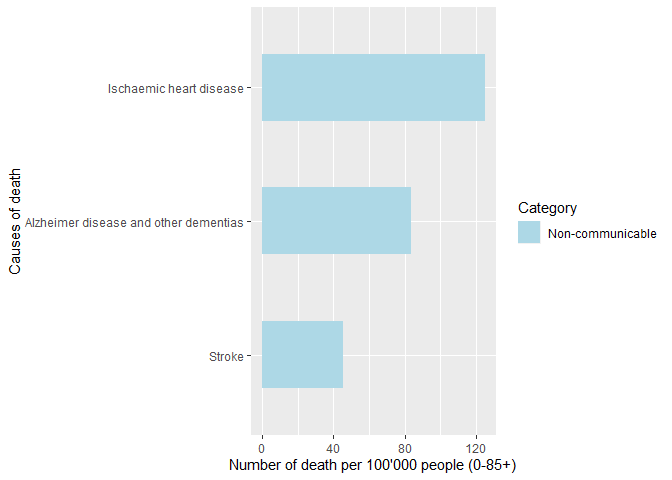
\includegraphics{Scientific-report-2022---CS_files/figure-latex/unnamed-chunk-4-1.pdf}

In this graph, we can see that the three most common deaths for all
groups are ischaemic heart disease (cause n°1), Alzheimer disease and
other dementia (cause n°2), and stroke (cause n°3). All of these causes
are considered ``non-communicable''.

What is this telling us ? First of all, let's take a look at the number
of death per 100'000 people between ages :

\begin{Shaded}
\begin{Highlighting}[]
\NormalTok{DeathADCH }\OtherTok{\textless{}{-}}\NormalTok{ Deathstat[}\DecValTok{4}\SpecialCharTok{:}\DecValTok{60}\NormalTok{,]}

\FunctionTok{ggplot}\NormalTok{(DeathADCH, }\FunctionTok{aes}\NormalTok{(}\AttributeTok{x=}\FunctionTok{fct\_relevel}\NormalTok{(Age, }\FunctionTok{c}\NormalTok{(}\StringTok{"5{-}9"}\NormalTok{), }\AttributeTok{after =} \DecValTok{2}\NormalTok{), }\AttributeTok{y=}\NormalTok{Nb)) }\SpecialCharTok{+}
  \FunctionTok{geom\_point}\NormalTok{(}\AttributeTok{color=}\StringTok{"Lightblue"}\NormalTok{, }\AttributeTok{size=}\DecValTok{4}\NormalTok{, }\AttributeTok{alpha=}\FloatTok{0.6}\NormalTok{) }\SpecialCharTok{+} 
  \FunctionTok{geom\_segment}\NormalTok{(}\FunctionTok{aes}\NormalTok{(}\AttributeTok{x=}\NormalTok{Age, }\AttributeTok{xend=}\NormalTok{Age, }\AttributeTok{y=}\DecValTok{0}\NormalTok{, }\AttributeTok{yend=}\NormalTok{Nb)) }\SpecialCharTok{+}
  \FunctionTok{theme\_light}\NormalTok{() }\SpecialCharTok{+}
  \FunctionTok{coord\_flip}\NormalTok{() }\SpecialCharTok{+}
  \FunctionTok{xlab}\NormalTok{(}\StringTok{"Age groups"}\NormalTok{) }\SpecialCharTok{+}
  \FunctionTok{ylab}\NormalTok{(}\StringTok{"Number of death per 100\textquotesingle{}000 people (0{-}85+)"}\NormalTok{) }\SpecialCharTok{+}
  \FunctionTok{theme}\NormalTok{(}
    \AttributeTok{panel.grid.major.y =} \FunctionTok{element\_blank}\NormalTok{(),}
    \AttributeTok{panel.border =} \FunctionTok{element\_blank}\NormalTok{(),}
    \AttributeTok{axis.ticks.y =} \FunctionTok{element\_blank}\NormalTok{())}
\end{Highlighting}
\end{Shaded}

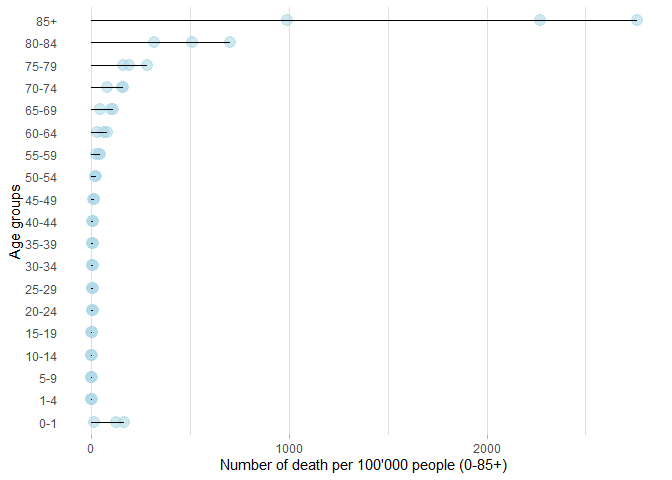
\includegraphics{Scientific-report-2022---CS_files/figure-latex/unnamed-chunk-5-1.pdf}

What we can see is that the number of death per 100'000 people is quite
high for children between 0 and 1 years-old, compared to people between
1 and 49 years-old. Then, the number increase from 50 years-old and
reach the highest for the 85 years-old and more.

That explains why the three main causes of death across all ages in
Switzerland in 2019 is composed only of non-communicable diseases.

\hypertarget{statistical-tests}{%
\subsubsection{Statistical tests}\label{statistical-tests}}

\begin{Shaded}
\begin{Highlighting}[]
\NormalTok{TestLM }\OtherTok{\textless{}{-}} \FunctionTok{lm}\NormalTok{(Nb}\SpecialCharTok{\textasciitilde{}}\NormalTok{Age, }\AttributeTok{data =}\NormalTok{ Deathstat)}
\FunctionTok{summary}\NormalTok{(TestLM)}
\end{Highlighting}
\end{Shaded}

\begin{verbatim}
## 
## Call:
## lm(formula = Nb ~ Age, data = Deathstat)
## 
## Residuals:
##      Min       1Q   Median       3Q      Max 
## -1017.70    -2.15    -0.14     4.28   754.04 
## 
## Coefficients:
##             Estimate Std. Error t value Pr(>|t|)    
## (Intercept)   102.22     121.81   0.839   0.4064    
## Age0-85+      -17.55     172.27  -0.102   0.9193    
## Age1-4       -100.67     172.27  -0.584   0.5623    
## Age10-14     -101.46     172.27  -0.589   0.5592    
## Age15-19      -99.36     172.27  -0.577   0.5673    
## Age20-24      -98.22     172.27  -0.570   0.5717    
## Age25-29      -97.73     172.27  -0.567   0.5737    
## Age30-34      -98.01     172.27  -0.569   0.5726    
## Age35-39      -96.73     172.27  -0.562   0.5776    
## Age40-44      -95.21     172.27  -0.553   0.5836    
## Age45-49      -90.52     172.27  -0.525   0.6022    
## Age5-9       -101.57     172.27  -0.590   0.5588    
## Age50-54      -82.03     172.27  -0.476   0.6365    
## Age55-59      -67.09     172.27  -0.389   0.6990    
## Age60-64      -45.76     172.27  -0.266   0.7919    
## Age65-69      -16.82     172.27  -0.098   0.9227    
## Age70-74       30.52     172.27   0.177   0.8603    
## Age75-79      109.09     172.27   0.633   0.5302    
## Age80-84      405.04     172.27   2.351   0.0237 *  
## Age85+       1903.87     172.27  11.052 9.99e-14 ***
## ---
## Signif. codes:  0 '***' 0.001 '**' 0.01 '*' 0.05 '.' 0.1 ' ' 1
## 
## Residual standard error: 211 on 40 degrees of freedom
## Multiple R-squared:  0.866,  Adjusted R-squared:  0.8023 
## F-statistic:  13.6 on 19 and 40 DF,  p-value: 6.188e-12
\end{verbatim}

\begin{Shaded}
\begin{Highlighting}[]
\FunctionTok{anova}\NormalTok{(TestLM)}
\end{Highlighting}
\end{Shaded}

\begin{verbatim}
## Analysis of Variance Table
## 
## Response: Nb
##           Df   Sum Sq Mean Sq F value    Pr(>F)    
## Age       19 11504105  605479  13.602 6.188e-12 ***
## Residuals 40  1780590   44515                      
## ---
## Signif. codes:  0 '***' 0.001 '**' 0.01 '*' 0.05 '.' 0.1 ' ' 1
\end{verbatim}

\begin{Shaded}
\begin{Highlighting}[]
\CommentTok{\# (F{-}statistic = 13.602, df = 19, 40), p{-}value \textless{} .001)}
\CommentTok{\# The effect of age is significant}
\end{Highlighting}
\end{Shaded}

To have a better understanding of the different causes, we will now look
at the three main causes of death among children and young-adults, to
see, later, if there is a difference compared to adults.

\hypertarget{causes-of-deaths-among-infants-0-19-years-old}{%
\section{Causes of deaths among infants (0-19
years-old)}\label{causes-of-deaths-among-infants-0-19-years-old}}

Here is a graph that present the type of death that we can find among
children between 0 and 19 years-old. This graph confirm our hypothesis
that children die mostly from communicable and non-communicable
diseases.

\begin{Shaded}
\begin{Highlighting}[]
\NormalTok{DeathInfant }\OtherTok{\textless{}{-}}\NormalTok{Deathstat[}\DecValTok{4}\SpecialCharTok{:}\DecValTok{18}\NormalTok{,]}

\FunctionTok{ggplot}\NormalTok{(DeathInfant, }\FunctionTok{aes}\NormalTok{(}\AttributeTok{x=}\NormalTok{Nb, }\AttributeTok{y=}\NormalTok{Cause, }\AttributeTok{fill=}\NormalTok{Category, }\AttributeTok{width =} \FloatTok{0.5}\NormalTok{)) }\SpecialCharTok{+}
  \FunctionTok{geom\_bar}\NormalTok{(}\AttributeTok{stat =} \StringTok{"identity"}\NormalTok{) }\SpecialCharTok{+}
  \FunctionTok{xlab}\NormalTok{(}\StringTok{"Number of death per 100\textquotesingle{}000 people (0{-}19)"}\NormalTok{) }\SpecialCharTok{+} 
  \FunctionTok{ylab}\NormalTok{(}\StringTok{"Causes of death"}\NormalTok{)}
\end{Highlighting}
\end{Shaded}

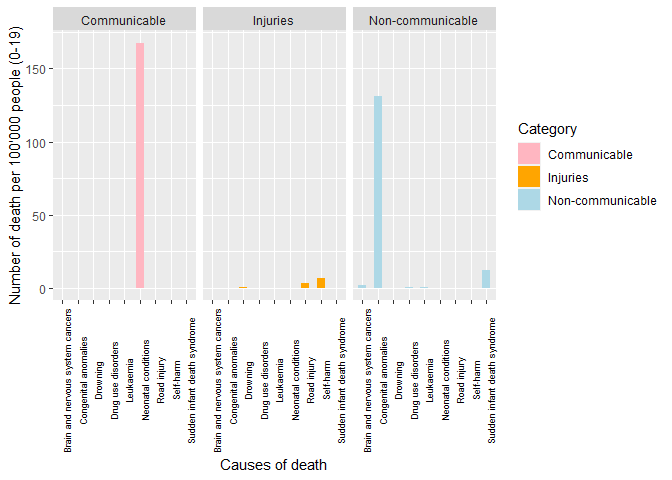
\includegraphics{Scientific-report-2022---CS_files/figure-latex/unnamed-chunk-7-1.pdf}

However, we saw earlier that there are more deaths among the 0-1
years-old compared to the 1-19 years-old. What happen if we compared
causes of deaths among children between 1 and 19 years-old ?

\hypertarget{causes-of-deaths-between-ages-in-children}{%
\subsection{Causes of deaths between ages in
children}\label{causes-of-deaths-between-ages-in-children}}

\begin{Shaded}
\begin{Highlighting}[]
\NormalTok{DeathChild }\OtherTok{\textless{}{-}}\NormalTok{ Deathstat[}\DecValTok{7}\SpecialCharTok{:}\DecValTok{18}\NormalTok{,]}

\FunctionTok{ggplot}\NormalTok{(DeathChild, }\FunctionTok{aes}\NormalTok{(}\AttributeTok{x=}\FunctionTok{fct\_relevel}\NormalTok{(Age, }\FunctionTok{c}\NormalTok{(}\StringTok{"5{-}9"}\NormalTok{), }\AttributeTok{after =} \DecValTok{1}\NormalTok{), }\AttributeTok{y=}\NormalTok{Nb, }\AttributeTok{fill=}\NormalTok{Category, }\AttributeTok{width=}\FunctionTok{c}\NormalTok{(}\FloatTok{0.2}\NormalTok{))) }\SpecialCharTok{+}
  \FunctionTok{geom\_bar}\NormalTok{(}\AttributeTok{stat =} \StringTok{"identity"}\NormalTok{) }\SpecialCharTok{+}
  \FunctionTok{xlab}\NormalTok{(}\StringTok{"Age groups"}\NormalTok{) }\SpecialCharTok{+} 
  \FunctionTok{ylab}\NormalTok{(}\StringTok{"Number of death per 100\textquotesingle{}000 people (1{-}19)"}\NormalTok{)}
\end{Highlighting}
\end{Shaded}

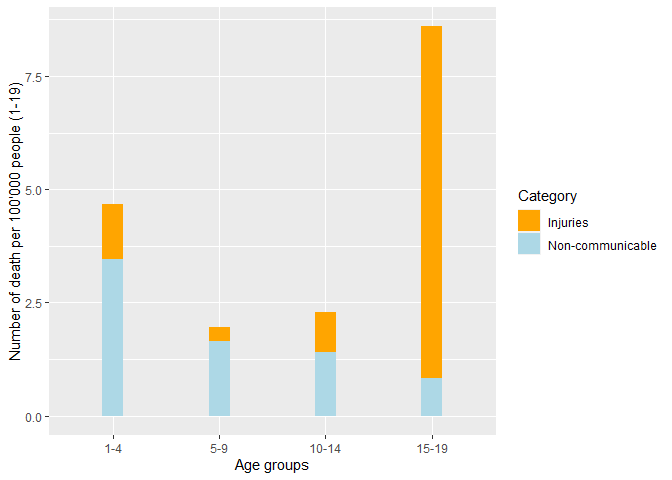
\includegraphics{Scientific-report-2022---CS_files/figure-latex/unnamed-chunk-8-1.pdf}

What we see in this graph confirms our hypothesis that children from 0
to 14 die mosly from communicable and non-communicable disease, and that
young adults mostly die from injuries. Now that we confirmed our
hypothesis with children and young-adults, lets take a look at the
causes of deaths among adults to see if there is a difference between
adults and children.

\hypertarget{causes-of-deaths-among-adults}{%
\section{Causes of deaths among
adults}\label{causes-of-deaths-among-adults}}

\begin{Shaded}
\begin{Highlighting}[]
\NormalTok{DeathAdult }\OtherTok{\textless{}{-}}\NormalTok{ Deathstat[}\DecValTok{19}\SpecialCharTok{:}\DecValTok{57}\NormalTok{,]}

\FunctionTok{ggplot}\NormalTok{(DeathAdult, }\FunctionTok{aes}\NormalTok{(}\AttributeTok{x=}\NormalTok{Age, }\AttributeTok{y=}\NormalTok{Nb, }\AttributeTok{fill=}\NormalTok{Category, }\AttributeTok{width=}\FunctionTok{c}\NormalTok{(}\FloatTok{0.1}\NormalTok{))) }\SpecialCharTok{+}
  \FunctionTok{geom\_bar}\NormalTok{(}\AttributeTok{stat =} \StringTok{"identity"}\NormalTok{) }\SpecialCharTok{+}
  \FunctionTok{xlab}\NormalTok{(}\StringTok{"Age groups"}\NormalTok{) }\SpecialCharTok{+} 
  \FunctionTok{ylab}\NormalTok{(}\StringTok{"Number of death per 100\textquotesingle{}000 people"}\NormalTok{)}
\end{Highlighting}
\end{Shaded}

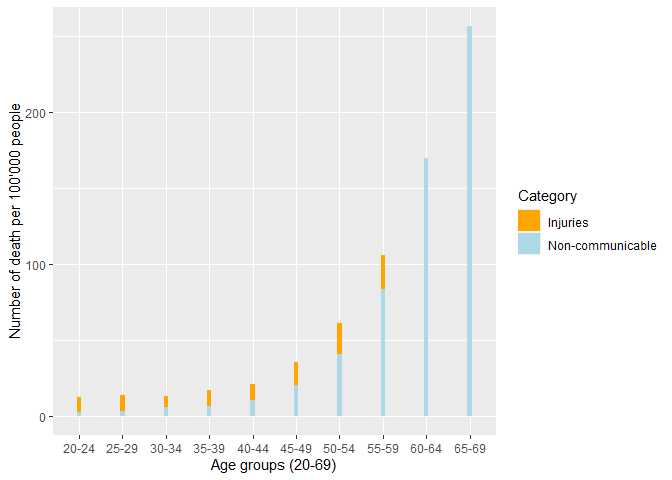
\includegraphics{Scientific-report-2022---CS_files/figure-latex/unnamed-chunk-9-1.pdf}

To have a better view, let's take only adults between 20 and 69, given
the fact that there are more deaths after 75 year-old and what we see in
the begining, in is only non-communicable diseases :

\begin{Shaded}
\begin{Highlighting}[]
\NormalTok{DeathAdult2 }\OtherTok{\textless{}{-}}\NormalTok{ Deathstat[}\DecValTok{19}\SpecialCharTok{:}\DecValTok{48}\NormalTok{,]}

\FunctionTok{ggplot}\NormalTok{(DeathAdult2, }\FunctionTok{aes}\NormalTok{(}\AttributeTok{x=}\NormalTok{Age, }\AttributeTok{y=}\NormalTok{Nb, }\AttributeTok{fill=}\NormalTok{Category, }\AttributeTok{width=}\FunctionTok{c}\NormalTok{(}\FloatTok{0.1}\NormalTok{))) }\SpecialCharTok{+}
  \FunctionTok{geom\_bar}\NormalTok{(}\AttributeTok{stat =} \StringTok{"identity"}\NormalTok{) }\SpecialCharTok{+}
  \FunctionTok{xlab}\NormalTok{(}\StringTok{"Age groups (20{-}69)"}\NormalTok{) }\SpecialCharTok{+} 
  \FunctionTok{ylab}\NormalTok{(}\StringTok{"Number of death per 100\textquotesingle{}000 people"}\NormalTok{)}
\end{Highlighting}
\end{Shaded}

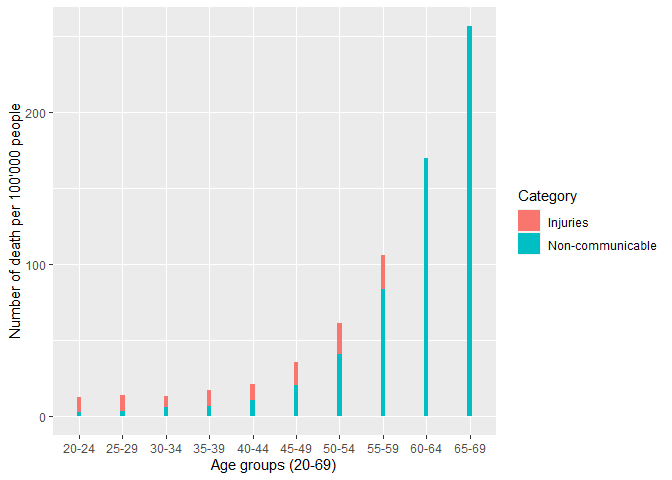
\includegraphics{Scientific-report-2022---CS_files/figure-latex/unnamed-chunk-10-1.pdf}

What we can see is that :

\hypertarget{conclusion}{%
\section{Conclusion}\label{conclusion}}

Children between 0-14 died mosly of communicable disease. Children and
Adults between 15 - 49 die mosly of injuries. Then, people betweem 0-1
and between 40 and 85+ die mostly from non-communicable disease.

\hypertarget{references}{%
\section{References}\label{references}}

\end{document}
